\documentclass[10pt,a4paper]{article}
\usepackage[natbibapa]{apacite} 
\usepackage{amsmath}
\usepackage{tikz}
\usepackage{physics}
\usepackage[a4paper,margin=1.2in]{geometry} 
\bibliographystyle{apacite}


\title{Assignment 2 Machine Learning COS4852}
\author{ Adriaan Louw (53031377) }

\tikzset{
  treenode/.style = {shape=rectangle, rounded corners,
                     draw, align=center,
                     top color=white, bottom color=blue!20},
  root/.style     = {treenode, font=\Large, bottom color=red!30},
  env/.style      = {treenode, font=\ttfamily\normalsize},
  dummy/.style    = {circle,draw}
}

\newcommand{\eeq}[1]{\begin{equation}
\begin{split}
#1
\end{split}
\end{equation}}

\usetikzlibrary{shapes.misc}
\usetikzlibrary{decorations.pathreplacing}

\tikzset{cross/.style={cross out, draw=black, minimum size=20*(#1-\pgflinewidth), inner sep=0pt, outer sep=0pt}, 
%default radius will be 1pt. 
cross/.default={1pt}}


\tikzset{basic/.style={draw,fill=blue!50!green!20,
                       text badly centered,minimum width=3em}}
\tikzset{input/.style={basic,circle}}
\tikzset{weights/.style={basic,rectangle,minimum width=2em}}
\tikzset{functions/.style={basic,circle,fill=blue!50!green!20}}
\newcommand{\addsymbol}{\draw[thick] (0.5em,0.5em) -- (0,0.5em) -- 
                        (0,-0.5em) --  (-0.5em,-0.5em)
                        (0em,0.75em) -- (0em,-0.75em)
                        (0.75em,0em) -- (-0.75em,0em);}
\begin{document}

\maketitle

\tableofcontents

\section{Question 1}
\subsection{Question 1(a)}

Firstly we calculate the line 

\begin{equation}
\label{line}
 x_2 = mx_1 + c
\end{equation}

for the intersect points (2,0) and (0,6).

Calculating slope m,

\begin{equation}
\begin{split}
m &= \frac{6-0}{0-2} \\
  &= -3\\
\end{split}
\end{equation}

$x_2$ intercept $c$ is 6.

This makes equation \ref{line}

\begin{equation}
\label{pop}
x_2 = -3x_1 + 6
\end{equation}

\cite{nils} gives the equation for the hyperplane as

\begin{equation}
\sum_{i=1}^n x_i\omega_i \geq \theta
\end{equation}

which in this case gives the equation for the hyperplane to be

\begin{equation}
\label{weightline}
\omega_1x_1 + \omega_2x_2 +\omega_3 = 0
\end{equation}

We need to get equation \ref{weightline} in the form of equation \ref{line}

\begin{equation}
\begin{split}
\label{simp}
\omega_1x_1 + \omega_2x_2 + +\omega_3 &= 0\\
\omega_2x_2 &= -\omega_1x_1 - \omega_3\\ 
x_2 &= -\frac{\omega_1x_1}{\omega_2} - \frac{\omega_3}{\omega_2} \\ 
\end{split}
\end{equation}

Comparing coefficients m and c from equation \ref{pop} to \ref{simp} we get

\begin{equation}
\begin{split}
-\frac{\omega_1}{\omega_2} &= -3 \\
\omega_1 &= 3\omega_2\\ 
\end{split}
\end{equation}

and

\begin{equation}
\begin{split}
-\frac{\omega_3}{\omega_2} &= 6\\
\omega_3 &= -6\omega_2\\ 
\end{split}
\end{equation}

If we choose $\omega_3 = -2$ then $\omega_1=1$ and $\omega_2 = \frac{1}{3}$. This makes the hyperplane equation from equation \ref{weightline}

\begin{equation}
x_1 + \frac{x_2}{3} -2 = 0
\end{equation}

Now we need to test this hyperplane. For positive instance (2,6)

\begin{equation}
\begin{split}
x_1 + \frac{x_2}{3} - 2 &= \\
2 + \frac{6}{2} - 2 &= \\
2&\\
\end{split}
\end{equation}

Which is as expected.

And the negative instance (-1,2)

\begin{equation}
\begin{split}
x_1 + \frac{x_2}{3} - 2 &= \\
-1 + \frac{2}{3} -2 & = \\
-\frac{7}{3}
\end{split}
\end{equation}

This is also as expected. The perceptron now classifies the the data correctly
\subsection{Question 1(b)}

\begin{center}
\begin{tikzpicture}[scale=0.6]
%\draw [help lines] (-3,-3) grid (3,3);
% Euclidean
\draw [<->](0,-8)--(0,8) node[right]{$X_2$};
\draw [<->](-8,0)--(8,0) node[right]{$X_1$};
 
%labels
\foreach \x in {-8,-6,-4,-2,2,4,6,8}
     \draw (\x,1pt) -- (\x,-3pt) node[anchor=north] {$\x$};

\foreach \y/\ytext in {-8,-6,-4,-2,2,4,6,8}
     \draw (1pt,\y) -- (-3pt,\y) node[anchor=east] {$\y$};
 
\draw (-1,2) node[cross,green]{};
\draw (1,-2) node[cross,green]{};
\draw (-2,-5) node[cross,green]{};
\draw (-5,-2) node[cross,green]{}; 

\draw (-5,6) node[cross,red]{};
\draw (3,5) node[cross,red]{};
\draw (2,-2) node[cross,red]{};
\draw (5,-5) node[cross,red]{};

\draw [blue] (-8,8) -- (8,-8);
\draw [teal] (-8,66/7) -- (8,-62/7);
 
\end{tikzpicture}
\end{center}

From the above image we can see that any that it is not possible to create a hyperplane that correctly classifies all negative instances and positive instances. The blue line is the line $x_2 = -x_1$ and the teal line is the line $x_2 = -\frac{7}{8}x_1 + \frac{2}{7}$. The any minimum plane that correctly classifies all the negative instances will classify the positive instance (-1,2) incorrectly as negative. 

We can create a hyperplane from regression from all the points close to where the hyperplane should be. Using negative points (-5,6),(2,-2),(5,-5) and positive points (-1,2),(1,-2)

For the equation of the regressed line $x_2=mx_1+c$

\begin{equation}
\begin{split}
\label{m}
m &= r\frac{S(x_2)}{S(x_1)}\\ 
m &= \frac{\sum((x_1 - \bar{x_1})(x_2-\bar{x_2}))}{\sqrt{\sum (x_1-\bar{x_1})^2 \sum(x_2-\bar{x_2})^2}} \frac{\sqrt{\frac{\sum (x_2-\bar{x_2})^2}{n-1}}}{\sqrt{\frac{\sum (x_1-\bar{x_1})^2}{n-1}}}\\
\end{split}
\end{equation}

where r is Pearsons Correlation Coefficient and S is standard deviation of axis $x_2$ or $x_1$.

Here follows the calculation

\begin{tabular}{|c|c|c|c|c|c|c|}
\hline
$x_1$ & $x_2$ & $x_1-\bar{x_1}$ & $x_2-\bar{x_2}$ &$(x_1-\bar{x_1})(x_2-\bar{x_2})$ & $(x_1-\bar{x_1})^2$ & $(x_2-\bar{x_2})^2$ \\ 
\hline
-5 &  6 & -5.4 &  6.2 & -33.48 & 29.16 & 38.44\\
 2 & -2 &  1.6 & -1.8 &  -2.88 &  2.56 &  3.24\\
 5 & -5 &  4.6 & -4.8 & -22.08 & 21.16 & 23.04\\
-1 &  2 & -1.4 &  2.2 &  -3.08 &  1.96 &  4.84\\
 1 & -2 &  0.6 & -1.8 &  -1.08 &  0.36 &  3.24\\
\hline
\end{tabular}

From the above table we have $\bar{x_1} = 0.4, \bar{x_2} = -0.2, \sum((x_1 - \bar{x_1})(x_2-\bar{x_2})) = -62.6, (x_1-\bar{x_1})^2 = 55.2,and (x_2-\bar{x_2})^2 = 72.8$ 

Passing these into equation \ref{m} we get m = -1.13

\begin{equation}
\begin{split}
c &= \bar{x_2} - m\bar{x_1}\\
  &= -0.2 - (-1.13)(0.4)\\
  &= 0.25\\  
\end{split}
\end{equation}

Which gives us equation 

\begin{equation}
x_2 = -1.13x_1 + 0.25
\end{equation}

Visually it would be

\begin{center}
\begin{tikzpicture}[scale=0.6]
%\draw [help lines] (-3,-3) grid (3,3);
% Euclidean
\draw [<->](0,-8)--(0,8) node[right]{$X_2$};
\draw [<->](-8,0)--(8,0) node[right]{$X_1$};
 
%labels
\foreach \x in {-8,-6,-4,-2,2,4,6,8}
     \draw (\x,1pt) -- (\x,-3pt) node[anchor=north] {$\x$};

\foreach \y/\ytext in {-8,-6,-4,-2,2,4,6,8}
     \draw (1pt,\y) -- (-3pt,\y) node[anchor=east] {$\y$};
 
\draw (-1,2) node[cross,green]{};
\draw (1,-2) node[cross,green]{};
\draw (-2,-5) node[cross,green]{};
\draw (-5,-2) node[cross,green]{}; 

\draw (-5,6) node[cross,red]{};
\draw (3,5) node[cross,red]{};
\draw (2,-2) node[cross,red]{};
\draw (5,-5) node[cross,red]{};

\draw [blue] (-8,9.32) -- (8,-8.81);
 
\end{tikzpicture}
\end{center}

This will minimise the error even though it would incorrectly classify (-1,2)

\subsection{Question 1(c)}

The equation for the hyperplane is: 

\begin{equation}
\label{3d}
\omega_1 x_1 + \omega_2 x_2 + \omega_3 x_3 + \omega_0 = 0
\end{equation}

Passing in the point (14.0,0) gives us into equation \ref{3d}
\begin{equation}
\begin{split}
\omega_1 x_1 + \omega_2 x_2 + \omega_3 x_3 + \omega_0 &= 0 \\
\omega_1(14) + \omega_2(0) + \omega_3(0) + \omega_0 &=0\\
14\omega_1 + \omega_0 &= 0\\
\omega_1 &= -\frac{\omega_0}{14}\\
\end{split}
\end{equation}

Passing the point (0,8,0) into equation \ref{3d}
\begin{equation}
\begin{split}
\omega_1 x_1 + \omega_2 x_2 + \omega_3 x_3 + \omega_0 &= 0 \\
\omega_1(0) + \omega_2(8) + \omega_3(0) + \omega_0 &=0\\
8\omega_2 + \omega_0 &= 0\\
\omega_2 &= -\frac{\omega_0}{8}\\
\end{split}
\end{equation}

Passing the point (0,0,6) into equation \ref{3d}
\begin{equation}
\begin{split}
\omega_1 x_1 + \omega_2 x_2 + \omega_3 x_3 + \omega_0 &= 0 \\
\omega_1(0) + \omega_2(0) + \omega_3(6) + \omega_0 &=0\\
6\omega_3 + \omega_0 &= 0\\
\omega_3 &= -\frac{\omega_0}{6}\\
\end{split}
\end{equation}

Now we need to solve the 3 simultaneous equations. Any value of $\omega_0$ will solve the equation but we still need to check for polarity

If $\omega_0 = -1$

Then $\omega_1 = \frac{1}{14}$,$\omega_2=\frac{1}{8}$ and $\omega_3 = \frac{1}{6}$.

Checking for polarity with positive instance (3,5,5)

\begin{equation}
\begin{split}
\omega_1 x_1 + \omega_2 x_2 + \omega_3 x_3 + \omega_0 &= \\
\frac{1}{14}(3) + \frac{1}{8}(5) + \frac{1}{6}(5) -1 &= \\
\frac{36 + 105 + 140 -168}{168} &= \\
\frac{113}{168}\\
\end{split}
\end{equation}

Which is positive thus meaning the polarity is correct.

Thus $\omega_0 = -1; \omega_1 = \frac{1}{14} ; \omega_2=\frac{1}{8}; \omega_3 = \frac{1}{6}$.

\subsection{Question 1(d)}

  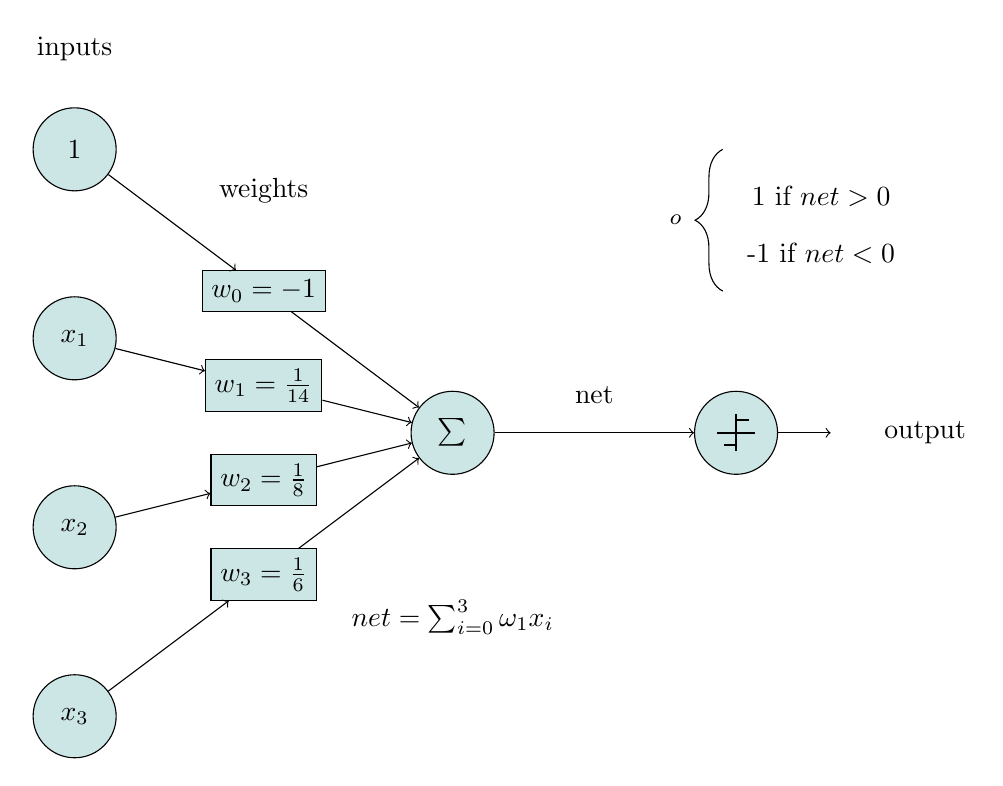
\begin{tikzpicture}[scale=1.2]
    \foreach \h [count=\hi ] in {$x_3$,$x_2$,$x_1$,$1$}{%
          \node[input] (f\hi) at (0,\hi*2cm-5 cm) {\h};
        }
    \node[functions] (sum) at (4,0) {$\sum$};
    \foreach \h [count=\hi ] in {$w_3=\frac{1}{6}$,$w_2=\frac{1}{8}$,$w_1=\frac{1}{14}$,$w_0=-1$}{%
          \path (f\hi) -- node[weights] (w\hi) {\h} (sum);
          \draw[->] (f\hi) -- (w\hi);
          \draw[->] (w\hi) -- (sum);
        }        
    \node[functions] (step) at (7,0) {};
       \begin{scope}[xshift=7cm,scale=.75]
         \addsymbol
       \end{scope}
    \draw[->] (sum) -- (step);
    \draw[->] (step) -- ++(1,0);
    % Labels
    \node[above=1cm] at (f4) {inputs};
    \node[above=1cm] at (w4) {weights};
    \node at (5.5,0.4) {net};
    \node[below=2cm] at (sum){$net = \sum_{i=0}^3 \omega_1 x_i$};
    \node at (9,0) {output};
    \draw [decorate,decoration={brace,amplitude=10pt},xshift=-4pt,yshift=0pt]
          (7.0,1.5) -- (7.0,3) node [black,midway,xshift=-0.6cm] 
          {\footnotesize $o$};
    \node at (7.9,2.5) {1 if $net > 0$};
    \node at (7.9,1.9) {-1 if $net < 0$};
    \end{tikzpicture}


\section{Question 2}
\subsection{Question 2(a)}

The truth table for this function is
 
\begin{tabular}{|c|c|c|c|}
\hline
$x_1$ & $x_2$ & $\neg x_1$ & $\neg x_1 \vee x_2$ \\
\hline
-1 &-1 &1 &-1\\
-1 &1 &1 &1\\
1 &-1 &-1 &-1\\
1 &1 &-1 &-1\\
\hline
\end{tabular}

Visually this is:

\begin{center}
\begin{tikzpicture}[scale=3.0]
%\draw [help lines] (-3,-3) grid (3,3);
% Euclidean
\draw [<->](0,-1.1)--(0,1.1) node[right]{$x_2$};
\draw [<->](-1.1,0)--(1.1,0) node[right]{$x_1$};
 
\draw[teal,thick,dashed] (-1.0,-0.5) -- (0.5,1.0);

%labels
\foreach \x in {-1,1}
     \draw (\x,1pt) -- (\x,-3pt) node[anchor=north] {$\x$};

\foreach \y/\ytext in {-1,1}
     \draw (1pt,\y) -- (-3pt,\y) node[anchor=east] {$\y$};
 
\draw (-1,-1) node[cross,red]{};
\draw (-1,1) node[cross,green]{};
\draw (1,-1) node[cross,red]{};
\draw (1,1) node[cross,red]{}; 

\end{tikzpicture}
\end{center}

The dashed line represents the function

\begin{equation}
x_2 = x_1 + 0.5
\end{equation}

This hyperplane will classify the boolean function correctly because it linearly separates all the positive instances from the negative ones.

The equation for the hyperplane with weights are given by equation \ref{weightline} and we know from equation \ref{simp} what the relationship is from the weight equation to the line equation. Thus for case

\begin{equation}
\begin{split}
m &= -\frac{\omega_1}{\omega_2} \\
1 &= -\frac{\omega_1}{\omega_2} \\
\omega_2 &= -\omega_1 \\
\end{split}
\end{equation}

and

\begin{equation}
\begin{split}
c &= -\frac{\omega_0}{\omega_2}\\
0.5 &= -\frac{\omega_0}{\omega_2}\\
\omega_0 &= -\frac{\omega_2}{2}\\
\end{split}
\end{equation}

Now we have the relationship between the weights. If we try $\omega_0 = 1$ we get $\omega_1 = 2$ and $\omega_2 = -2$ 

Which makes our weight equation

\begin{equation}
2x_1 - 2x_2 + 1
\end{equation}

Testing for polarity with point (-1,-1) we get
\begin{equation}
\begin{split}
2(-1) -2(-1) + 1 &= 1
\end{split}
\end{equation}

which indicates a positive result but we expect a negative result. Thus our polarity is wrong

We try $\omega_0 = -1$ which gives $\omega_1 = -2$ and $\omega_2 = 2$

Which makes the weight equation

\begin{equation}
-2x_1 + 2x_2 - 1
\end{equation}

Trying all our data we can sum it up in the following table

\begin{tabular}{|c|c|c|}
\hline
$x_1$ & $x_2$ & Result \\
\hline
-1 &-1 & -1\\
-1 & 1 & 4\\
1  &-1 & -5\\
1  & 1 & -1 \\
\hline
\end{tabular}

This shows that weights $\omega_0 = -1$; $\omega_1 = -2$ and $\omega_2 = 2$ correctly classify the data

 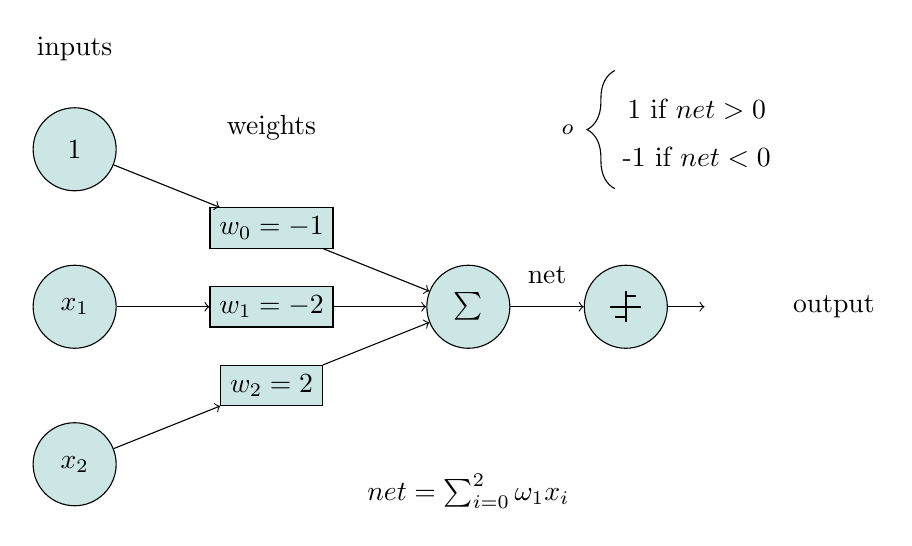
\begin{tikzpicture}[scale=1]
    \foreach \h [count=\hi ] in {$x_2$,$x_1$,$1$}{%
          \node[input] (f\hi) at (0,\hi*2cm-4 cm) {\h};
        }
    \node[functions] (sum) at (5,0) {$\sum$};
    \foreach \h [count=\hi ] in {$w_2 =2$,$w_1 = -2$,$w_0 = -1$}{%
          \path (f\hi) -- node[weights] (w\hi) {\h} (sum);
          \draw[->] (f\hi) -- (w\hi);
          \draw[->] (w\hi) -- (sum);
        }        

    \node[functions] (step) at (7,0) {};
       \begin{scope}[xshift=7cm,scale=.75]
         \addsymbol
       \end{scope}
    \draw[->] (sum) -- (step);
    \draw[->] (step) -- ++(1,0);
    % Labels
    \node[above=1cm]  at (f3) {inputs};
    \node[above=1cm] at (w3) {weights};
    \node[right=2cm] at (step) {output};
        \node at (6,0.4) {net};
    \node[below=2cm] at (sum){$net = \sum_{i=0}^2 \omega_1 x_i$};
    \draw [decorate,decoration={brace,amplitude=10pt},xshift=-4pt,yshift=0pt]
          (7.0,1.5) -- (7.0,3) node [black,midway,xshift=-0.6cm] 
          {\footnotesize $o$};
    \node at (7.9,2.5) {1 if $net > 0$};
    \node at (7.9,1.9) {-1 if $net < 0$};
    \end{tikzpicture}


















\subsection{Question 2(b)}

\begin{tabular}{|c|c|c|c|}
\hline
$x_1$ & $x_2$ & $x_1 \bigoplus x_2$ & $f_2 =\neg (x_1 \bigoplus x_2)$ \\
\hline
-1 &-1 &-1 &1\\
-1 &1 &1 &-1\\
1 &-1 &1 &-1\\
1 &1 &-1 &1\\
\hline
\end{tabular}

Visually this is:

\begin{center}
\begin{tikzpicture}[scale=3.0]
%\draw [help lines] (-3,-3) grid (3,3);
% Euclidean
\draw [<->](0,-1.1)--(0,1.1) node[right]{$x_2$};
\draw [<->](-1.1,0)--(1.1,0) node[right]{$x_1$};
 
\draw[red,thick,dashed] (-1.0,-0.5) -- (0.5,1.0);
\draw[red,thick,dashed] (-0.5,-1.0) -- (1.0,0.5);

%labels
\foreach \x in {-1,1}
     \draw (\x,1pt) -- (\x,-3pt) node[anchor=north] {$\x$};

\foreach \y/\ytext in {-1,1}
     \draw (1pt,\y) -- (-3pt,\y) node[anchor=east] {$\y$};
 
\draw (-1,-1) node[cross,green]{};
\draw (-1,1) node[cross,red]{};
\draw (1,-1) node[cross,red]{};
\draw (1,1) node[cross,green]{}; 

\end{tikzpicture}
\end{center}

We can see from the previous diagram that $f_2$ cannot be linearly separated by 1 hyperplane. In other words a single perceptron cannot classify this function. We need to try to decompose $f_2$ into multiple linearly separable functions that can be modelled by multiple perceptrons.

\begin{equation}
\begin{split}
f_2 &= \neg ( x_1 \bigoplus x_2 ) \\
    &= \neg( (x_1 \wedge \neg x_2) \vee (\neg x_1 \wedge x_2))\\
    &= \neg(x_1\wedge \neg x_2) \wedge \neg(\neg x_1 \wedge x_2)\\
    &= (\neg x_1 \vee x_2) \wedge (x_1 \vee \neg x_2)\\
\end{split}
\end{equation}  

We can thus create new function which is equivalent to $f_2$

\begin{equation}
g(h_1,h_2) = h_1 \wedge h_2 
\end{equation} 

where 

\begin{equation}
h_1 = \neg x_1 \vee x_2
\end{equation}

and 

\begin{equation}
h_2 = x_1 \vee \neg x_2
\end{equation}

The truth table will thus become

\begin{tabular}{|c|c|c|c|c|c|c|}
\hline
$x_1$ & $x_2$ & $x_1 \bigoplus x_2$ & $f_2 =\neg (x_1 \bigoplus x_2)$ & $h_1$ & $h_2$ &$g(h_1,h_2)$\\
\hline
-1 &-1 &-1 & 1 & 1 & 1 & 1  \\
-1 & 1 & 1 &-1 & 1 &-1 & -1 \\
 1 &-1 & 1 &-1 &-1 & 1 & -1 \\
 1 & 1 &-1 & 1 & 1 & 1 & 1  \\
\hline
\end{tabular}

Drawing $h_1$ gives

\begin{center}
\begin{tikzpicture}[scale=3.0]
%\draw [help lines] (-3,-3) grid (3,3);
% Euclidean
\draw [<->](0,-1.1)--(0,1.1) node[right]{$x_2$};
\draw [<->](-1.1,0)--(1.1,0) node[right]{$x_1$};
 
%\draw[red,thick,dashed] (-1.0,-0.5) -- (0.5,1.0);
\draw[red,thick,dashed] (-0.5,-1.0) -- (1.0,0.5);

%labels
\foreach \x in {-1,1}
     \draw (\x,1pt) -- (\x,-3pt) node[anchor=north] {$\x$};

\foreach \y/\ytext in {-1,1}
     \draw (1pt,\y) -- (-3pt,\y) node[anchor=east] {$\y$};
 
\draw (-1,-1) node[cross,green]{};
\draw (-1,1) node[cross,green]{};
\draw (1,-1) node[cross,red]{};
\draw (1,1) node[cross,green]{}; 

\end{tikzpicture}
\end{center}

Using equation \ref{weightline} and knowing this hyperplane goes through points (-0.5,-1) and (1.0,0.5).
We have  
\begin{equation}
\label{2bh1p1}
\begin{split}
\omega_1(-0.5) + \omega_2(-1) + \omega_0 &= 0 \\
\frac{-\omega_1}{2} - \omega_2 + \omega_0 &= 0 \\
\end{split}
\end{equation}
for the point (-0.5,-1) and

\begin{equation}
\label{2bh1p2}
\begin{split}
\omega_1(1) + \omega_2(0.5) + \omega_0 &= 0 \\
\omega_1 + \frac{\omega_2}{2} + \omega_0 &= 0 \\
\end{split}
\end{equation}

for point (1.0,0.5)

Equating equations \ref{2bh1p1} and \ref{2bh1p2} we get

\begin{equation}
\label{2bh1i}
\begin{split}
\frac{-\omega_1}{2} - \omega_2 + \omega_0 &= \omega_1 + \frac{\omega_2}{2} + \omega_0\\
\frac{3\omega_1}{2} &= \frac{3\omega_2}{2}\\
\omega_2 =& - \omega_1\\
\end{split}
\end{equation}

Passing equation \ref{2bh1i} into \ref{2bh1p2} we get

\begin{equation}
\begin{split}
\omega_1 + \frac{-\omega_1}{2} + \omega_0 &= 0 \\
\omega_0 &= -\frac{\omega_1}{2}\\
\end{split}
\end{equation}

If we take $\omega_0 = 1$ then $\omega_1 = -2$ and $\omega_2 = 2$.

Testing for polarity we use the point (-1,-1) where we expect a positive answer 

For point (-1,-1)

\begin{equation}
\begin{split}
-2x_1+2x_2 + 1 &=\\
-1(-1) + 2(-1) + 1& = 1\\
\end{split}
\end{equation}

Which is greater than 0 as expected. Thus the weights for $h_1$ is $\omega_0 = 1; \omega_1 = -2; \omega_2 = 2$ 

Now drawing $h_2$

\begin{center}
\begin{tikzpicture}[scale=3.0]
%\draw [help lines] (-3,-3) grid (3,3);
% Euclidean
\draw [<->](0,-1.1)--(0,1.1) node[right]{$x_2$};
\draw [<->](-1.1,0)--(1.1,0) node[right]{$x_1$};
 
\draw[red,thick,dashed] (-1.0,-0.5) -- (0.5,1.0);
%\draw[red,thick,dashed] (-0.5,-1.0) -- (1.0,0.5);

%labels
\foreach \x in {-1,1}
     \draw (\x,1pt) -- (\x,-3pt) node[anchor=north] {$\x$};

\foreach \y/\ytext in {-1,1}
     \draw (1pt,\y) -- (-3pt,\y) node[anchor=east] {$\y$};
 
\draw (-1,-1) node[cross,green]{};
\draw (-1,1) node[cross,red]{};
\draw (1,-1) node[cross,green]{};
\draw (1,1) node[cross,green]{}; 

\end{tikzpicture}
\end{center}

This is a similar perceptron from as in Question 2a. It uses the same hyperplane but the polarity is reversed. Thus from question 2a $\omega_2 = -\omega_1; \omega_0 = -\frac{\omega_2}{2}$. 

Testing polarity with $\omega_0 = 1$ then $\omega_1=2;\omega_2=-2$. This gives with positive instance (-1,-1)

\begin{equation}
\begin{split}
2x_1 - 2x_2 +1 &= \\
2(-1) - 2(-1) +1 &= 1 \\
\end{split}
\end{equation}  

Which indicates the preceptron calssifies the point (-1,-1) correctly as a positive instance

This means $\omega_0 = 1;\omega_1=2;\omega_2=-2$ for $h_2$


Now we need to create a perceptron for function g. The domain of g as a function of $h_1$ and $h_2$ can be shown as follows

\begin{center}
\begin{tikzpicture}[scale=3.0]
%\draw [help lines] (-3,-3) grid (3,3);
% Euclidean
\draw [<->](0,-1.1)--(0,1.1) node[right]{$h_2$};
\draw [<->](-1.1,0)--(1.1,0) node[right]{$h_1$};
 
\draw[red,thick,dashed] (1.1,-0.1) -- (-0.1,1.1);

%labels
\foreach \x in {-1,1}
     \draw (\x,1pt) -- (\x,-3pt) node[anchor=north] {$\x$};

\foreach \y/\ytext in {-1,1}
     \draw (1pt,\y) -- (-3pt,\y) node[anchor=east] {$\y$};
 
\draw (-1,1) node[cross,red]{};
\draw (1,-1) node[cross,red]{};
\draw (1,1) node[cross,green]{}; 

\end{tikzpicture}
\end{center}

From the above diagram we can see that a hyperplane through the points (0,1) and (1,0) will classify this perceptron

From applying equation \ref{weightline} to point $(h_1,h_2) = (1,0)$

\begin{equation}
\label{2bc1}
\begin{split}
\omega_1 x_1 + \omega_2 x_2 + \omega_0 &= 0 \\
\omega_1(1) + \omega_2(0) + \omega_0 &= 0 \\
\omega_1 &= -\omega_0\\
\end{split}
\end{equation}

and for point $(h_1,h_2) = (0,1)$

\begin{equation}
\label{2bc2}
\begin{split}
\omega_1 x_1 + \omega_2 x_2 + \omega_0 &= 0 \\
\omega_1(0) + \omega_2(1) + \omega_0 &= 0 \\
\omega_2 &= -\omega_0\\
\end{split}
\end{equation}

Now equation equations \ref{2bc1} and \ref{2bc2} we get $\omega_1 = \omega_2$

If we let $\omega_0 = -1$ then from substitution into equations \ref{2bc1} and \ref{2bc2} we get $\omega_1=\omega_2=1$.

Testing for polarity we have positive instance (1,1) 

\begin{equation}
\begin{split}
\omega_1 x_1 + \omega_2 x_2 + \omega_0 &= \\
x_1 + x_2 -1 &= \\
(1) + (1) - 1 &= 1
\end{split}
\end{equation}

Which is positive as expected

Figure \ref{fig} shows the whole network where $\omega_{1i}$ denotes the weights for the perceptron modeling $h_1$, $\omega_{2i}$ denotes the weights for the perceptron of $h_2$ and $\omega_{3i}$ denotes the weights of the final perceptron. 
\begin{figure}
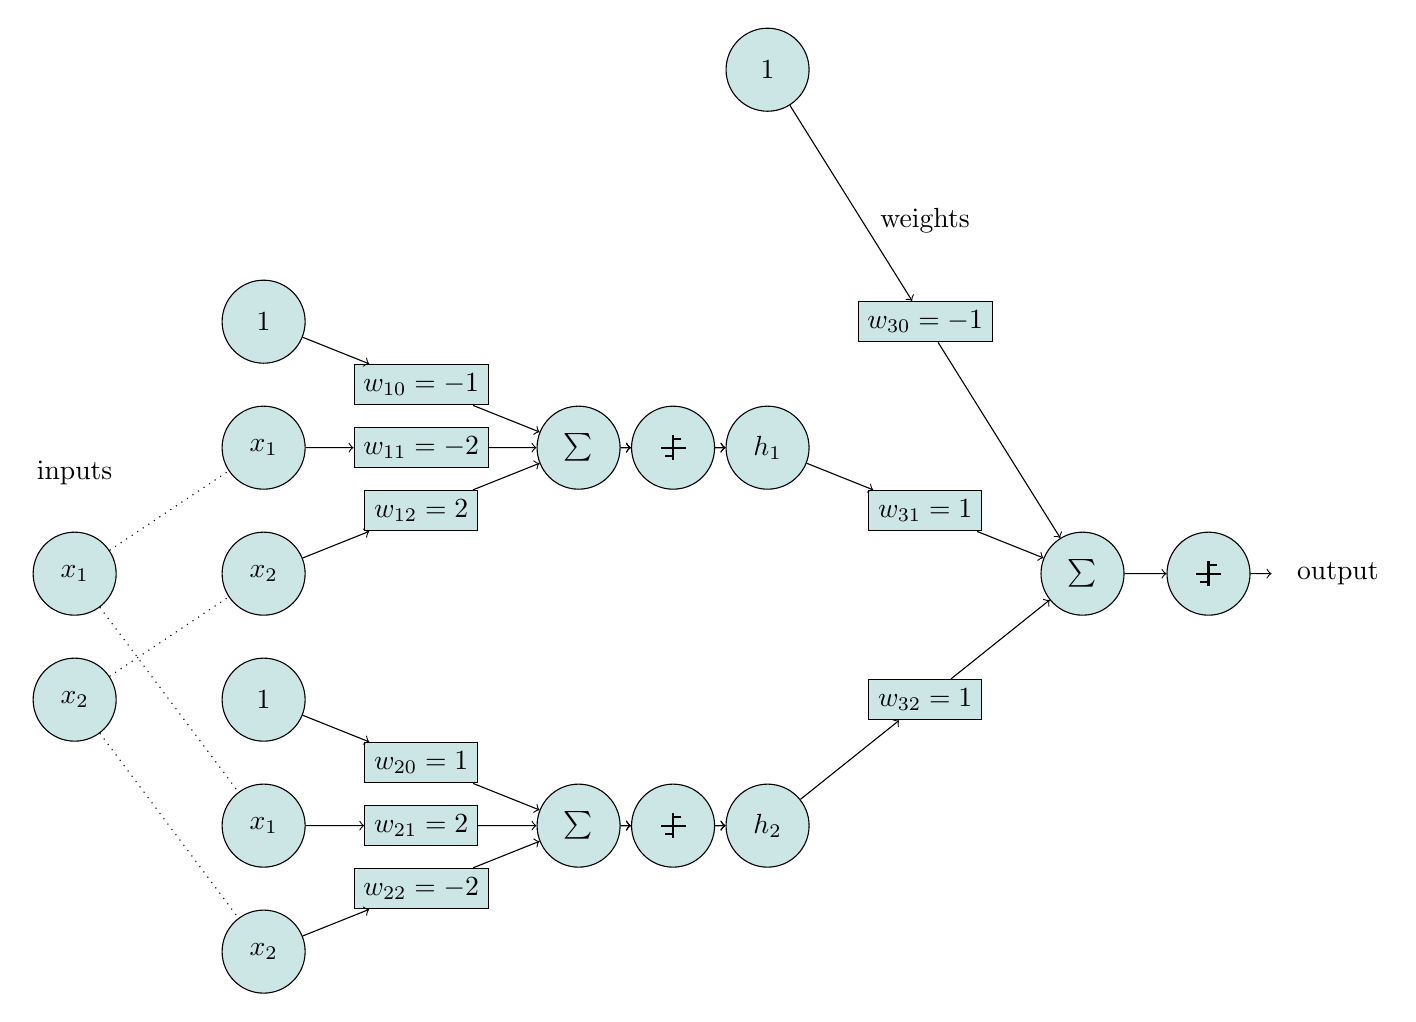
\begin{tikzpicture}[scale=0.8]

    %input x
    \node[input] (x1) at (-3,6){$x_1$};    
    \node[input] (x2) at (-3,4){$x_2$}; 

	% inputs of h1
    \foreach \h [count=\hi ] in {$x_2$,$x_1$,$1$}{
    	\node[input] (f1\hi) at (0,\hi*2cm +4cm) {\h};
    }
    % inputs of h2
    \foreach \h [count=\hi ] in {$x_2$,$x_1$,$1$}{
    	\node[input] (f2\hi) at (0,\hi*2cm -2cm) {\h};
    }
    
    \draw[dotted] (x1) -- (f12);    
    \draw[dotted] (x1) -- (f22);  
    \draw[dotted] (x2) -- (f11);    
    \draw[dotted] (x2) -- (f21);  
    
	% sum h1
	\node[functions] (sumh1) at (5,8) {$\sum$};
    % sum h2
	\node[functions] (sumh2) at (5,2) {$\sum$};
	
    \node[functions] (steph1) at (6.5,8) {};
       \begin{scope}[xshift=6.5cm,yshift=8cm,scale=.75]
         \addsymbol
       \end{scope}	
       
    \node[functions] (steph2) at (6.5,2) {};
       \begin{scope}[xshift=6.5cm,yshift=2cm,scale=.75]
         \addsymbol
       \end{scope}	
	
    % weights of h1
	\foreach \h [count=\hi ] in {$w_{12} =2$,$w_{11} = -2$,$w_{10} = -1$}{%
      	\path (f1\hi) -- node[weights] (w\hi) {\h} (sumh1);
      	\draw[->] (f1\hi) -- (w\hi);
      	\draw[->] (w\hi) -- (sumh1);
    } 
    % weights of h2
	\foreach \h [count=\hi ] in {$w_{22} =-2$,$w_{21} = 2$,$w_{20} = 1$}{%
      	\path (f2\hi) -- node[weights] (w\hi) {\h} (sumh2);
      	\draw[->] (f2\hi) -- (w\hi);
      	\draw[->] (w\hi) -- (sumh2);
    } 
	
	% inputs of g
	\foreach \h [count=\hi ] in {$h_2$,$h_1$,$1$}{%
      \node[input] (h\hi) at (8,\hi*6cm-4 cm) {\h};
    }
    % sum g
	\node[functions] (sumg) at (13,6) {$\sum$};
	% weights of g
	\foreach \h [count=\hi ] in {$w_{32} =1$,$w_{31} = 1$,$w_{30} = -1$}{%
      	\path (h\hi) -- node[weights] (w\hi) {\h} (sumg);
      	\draw[->] (h\hi) -- (w\hi);
      	\draw[->] (w\hi) -- (sumg);
      	\draw[->] (sumh1) -- (steph1);
      	\draw[->] (steph1) -- (h2);
      	\draw[->] (sumh2) -- (steph2);
      	\draw[->] (steph2) -- (h1);
    }        

    \node[functions] (stepg) at (15,6) {};
       \begin{scope}[xshift=15cm,yshift=6cm,scale=.75]
         \addsymbol
       \end{scope}
    
    \draw[->] (sumg) -- (stepg);       
	\draw[->] (stepg) -- ++(1,0);
	
	% Labels
	\node[above=1cm] at (x1) {inputs};
	\node[above=1cm] at (w3) {weights};
	\node[right=1cm] at (stepg) {output};
\end{tikzpicture}
\caption{Network for question 2b}
\label{fig}
\end{figure}

\subsection{Question 2(c)}

Given function

\begin{equation}
f_3(x_1,x_2) = (x_1 \vee x_2)\wedge(\neg x_1 \vee \neg x_2)
\end{equation}

The truth table for the function is the following:

\begin{tabular}{|c|c|c|c|c|c|c|}
\hline
$x_1$ & $x_2$ & $\neg x_1$ & $\neg x_2$ & $x_1 \vee x_2$ & $\neg x_1 \vee \neg x_2$ & $(x_1 \vee x_2)\wedge (\neg x_1 \vee \neg x_2)$\\
\hline
-1 &-1 &1 &1 & -1& 1 & -1\\
-1 &1 &1 &-1 & 1& 1 & 1\\
1 &-1 &-1 &1 & 1& 1 & 1\\
1 &1 &-1 &-1 & 1& -1 & -1\\
\hline
\end{tabular}


\begin{figure}
\begin{center}
\begin{tikzpicture}[scale=3.0]
%\draw [help lines] (-3,-3) grid (3,3);
% Euclidean
\draw [<->](0,-1.1)--(0,1.1) node[right]{$x_2$};
\draw [<->](-1.1,0)--(1.1,0) node[right]{$x_1$};
 
%\draw[red,thick,dashed] (-1.0,-0.5) -- (0.5,1.0);

%labels
\foreach \x in {-1,1}
     \draw (\x,1pt) -- (\x,-3pt) node[anchor=north] {$\x$};

\foreach \y/\ytext in {-1,1}
     \draw (1pt,\y) -- (-3pt,\y) node[anchor=east] {$\y$};
 
\draw (-1,-1) node[cross,red]{};
\draw (-1,1) node[cross,green]{};
\draw (1,-1) node[cross,green]{};
\draw (1,1) node[cross,red]{}; 

\end{tikzpicture}
\end{center}
\caption{Sketch of function $f_3(x_1,x_2)$} \label{fig2craw}
\end{figure}


Visually this can be seen in figure \ref{fig2craw}

No single hyperplane can classify all the data points. Multiple perceptrons will be needed. We will break the function up similar to Question 2b.

\begin{equation}
\begin{split}
f_3(x_1,x_2) &= g(h_1(x_1,x_2),h_2(x_1,x_2))\\
             &= h_1(x_1,x_2)\wedge h_2(x_1,x_2)\\
\end{split}
\end{equation}

where

\begin{equation}
h_1(x_1,x_2) = x_1\vee x_2
\end{equation}

and

\begin{equation}
h_2{x_1,x_2} = \neg x_1 \vee \neg x_2
\end{equation}

The truth table for $h_1(x_1,x_2)$ is:

\begin{tabular}{|c|c|c|}
\hline
$x_1$ & $x_2$ & $x_1 \vee x_2$ \\
\hline
-1 &-1 &-1 \\
-1 & 1 & 1 \\
 1 &-1 & 1 \\
 1 & 1 & 1 \\
\hline
\end{tabular}

Drawing the function $h_1(x_1,x_2)$ in Figure \ref{h1}

\begin{figure}
\begin{center}
\begin{tikzpicture}[scale=3.0]
%\draw [help lines] (-3,-3) grid (3,3);
% Euclidean
\draw [<->](0,-1.1)--(0,1.1) node[right]{$x_2$};
\draw [<->](-1.1,0)--(1.1,0) node[right]{$x_1$};
 
\draw[red,thick,dashed] (0.1,-1.1) -- (-1.1,0.1);

%labels
\foreach \x in {-1,1}
     \draw (\x,1pt) -- (\x,-3pt) node[anchor=north] {$\x$};

\foreach \y/\ytext in {-1,1}
     \draw (1pt,\y) -- (-3pt,\y) node[anchor=east] {$\y$};
 
\draw (-1,-1) node[cross,red]{};
\draw (-1,1) node[cross,green]{};
\draw (1,-1) node[cross,green]{};
\draw (1,1) node[cross,green]{}; 

\end{tikzpicture}
\end{center}
\caption{Sketch of function for $h_1(x_1,x_2)$ for Question 2c} \label{h1}
\end{figure}

We can see that $h_1$ will be classified by the hyperplane

\begin{equation}
x_2 = -x-1
\end{equation} 

Now we solve the weights equation (Eqn \ref{weightline}) with the points (0,-1) and (-1,0) on the hyperplane. Firstly with (0,-1)

\begin{equation}
\begin{split}
\omega_1 x_1 + \omega_2 x_2 \omega_0 &= 0\\
\omega_1 (0) + \omega_2 (-1) + \omega_0 &= 0\\
\omega_2 &= \omega_0\\
\end{split}
\end{equation}

and for point (-1,0)

\begin{equation}
\begin{split}
\omega_1 x_1 + \omega_2 x_2 \omega_0 &= 0\\
\omega_1 (-1) + \omega_2 (0) + \omega_0 &= 0\\
\omega_1 &= \omega_0\\
\end{split}
\end{equation}

Thus $\omega_0=\omega_1=\omega_2$. 

Since any value of $\omega_0$ will solve the equation, we try $\omega_0 = 1$. Now we test for polarity with negative instance (-1,-1).

\begin{equation}
\begin{split}
\omega_1 x_1 + \omega_2 x_2 \omega_0 &= \\
1(-1) +  1(-1) + 1 &= \\
-1\\
\end{split}
\end{equation}

The answer is negative thus correctly classifying the function $h_1(x_1,x_2)$

Now for the function $h_2(x_,x_2)$.

The truth table for $h_2(x_,x_2)$ is:

\begin{tabular}{|c|c|c|}
\hline
$x_1$ & $x_2$ & $\neg x_1 \vee \neg x_2$ \\
\hline
-1 &-1 & 1 \\
-1 & 1 & 1 \\
 1 &-1 & 1 \\
 1 & 1 &-1 \\
\hline
\end{tabular}

Drawing the function $h_1(x_1,x_2)$ in Figure \ref{h2}

\begin{figure}
\begin{center}
\begin{tikzpicture}[scale=3.0]
%\draw [help lines] (-3,-3) grid (3,3);
% Euclidean
\draw [<->](0,-1.1)--(0,1.1) node[right]{$x_2$};
\draw [<->](-1.1,0)--(1.1,0) node[right]{$x_1$};
 
\draw[red,thick,dashed] (-0.1,1.1) -- (1.1,-0.1);

%labels
\foreach \x in {-1,1}
     \draw (\x,1pt) -- (\x,-3pt) node[anchor=north] {$\x$};

\foreach \y/\ytext in {-1,1}
     \draw (1pt,\y) -- (-3pt,\y) node[anchor=east] {$\y$};
 
\draw (-1,-1) node[cross,green]{};
\draw (-1,1) node[cross,green]{};
\draw (1,-1) node[cross,green]{};
\draw (1,1) node[cross,red]{}; 

\end{tikzpicture}
\end{center}
\caption{Sketch of function for $h_2(x_1,x_2)$ for Question 2c} \label{h2}
\end{figure}

From Figure \ref{h2} we can see that function  $h_2(x_1,x_2)$ will be classified by the hyperplane

\begin{equation}
x_2 = -x_1 + 1
\end{equation} 

Now to solve the weights equation (Eqn \ref{weightline}) with the 2 points (0,1) and (1,0). For the point (0,1)

\begin{equation}
\begin{split}
\omega_1 x_1 + \omega_2 x_2 \omega_0 &= 0\\
\omega_1 (0) + \omega_2 (1) + \omega_0 &= 0\\
\omega_0 &= -\omega_2\\
\end{split}
\end{equation}

For the point (1,0)

\begin{equation}
\begin{split}
\omega_1 x_1 + \omega_2 x_2 \omega_0 &= 0\\
\omega_1 (1) + \omega_2 (0) + \omega_0 &= 0\\
\omega_0 &= -\omega_1\\
\end{split}
\end{equation}

Now any value of $\omega_0$ will solve this equation, but we need to check for polarity.

If we assume $\omega_0 = -1$  then $\omega_1=\omega_2=1$. We check with positive instance (-1,-1).

\begin{equation}
\begin{split}
\omega_1 x_1 + \omega_2 x_2 \omega_0 &= \\
1(-1) +  1(-1) + (-1) &= \\
-3\\
\end{split}
\end{equation}

Which gives a negative answer. Thus the polarity is swapped. Now trying $\omega_0 = 1$ and $\omega_1=\omega_2=-1$ with positive instance (-1,-1)

\begin{equation}
\begin{split}
\omega_1 x_1 + \omega_2 x_2 \omega_0 &= \\
-1(-1) +  -1(-1) + (1) &= \\
3\\
\end{split}
\end{equation}

$\omega_0 = 1$ correctly classifies the function $h_2(x_1,x_2)$

Now we need to determine the values of $g$ with respect to $h_1$ and $h_2$

\begin{tabular}{|c|c|c|c|c|c|c|}
\hline
$x_1$ & $x_2$ & $\neg x_1$ & $\neg x_2$ & $h_1 = x_1 \vee x_2$ & $h_2 = \neg x_1 \vee \neg x_2$ & $g=(x_1 \vee x_2)\wedge (\neg x_1 \vee \neg x_2)$\\
\hline
-1 &-1 &1 &1 & -1& 1 & -1\\
-1 &1 &1 &-1 & 1& 1 & 1\\
1 &-1 &-1 &1 & 1& 1 & 1\\
1 &1 &-1 &-1 & 1& -1 & -1\\
\hline
\end{tabular}

Now drawing the function $g_(h_1,h_2)$ in Figure \ref{g}. 

\begin{figure}
\begin{center}
\begin{tikzpicture}[scale=3.0]
%\draw [help lines] (-3,-3) grid (3,3);
% Euclidean
\draw [<->](0,-1.1)--(0,1.1) node[right]{$h_2$};
\draw [<->](-1.1,0)--(1.1,0) node[right]{$h_1$};
 
\draw[red,thick,dashed] (-0.1,1.1) -- (1.1,-0.1);

%labels
\foreach \x in {-1,1}
     \draw (\x,1pt) -- (\x,-3pt) node[anchor=north] {$\x$};

\foreach \y/\ytext in {-1,1}
     \draw (1pt,\y) -- (-3pt,\y) node[anchor=east] {$\y$};
 
\draw (-1,1) node[cross,red]{};
\draw (1,-1) node[cross,red]{};
\draw (1,1) node[cross,green]{}; 

\end{tikzpicture}
\end{center}
\caption{Sketch of function for $g(h_1,h_2)$ for Question 2c} \label{g}
\end{figure}

Note that the function $g_(h_1,h_2)$ is not defined for the point $(h_1,h_2)=(-1,-1)$.
This perceptron will be classified by the hyperplane

\begin{equation}
h_2 = -h_1 + 1
\end{equation}

Solving the weights equation (Eqn \ref{weightline}) for points $(h_1,h_2) = (0,1)$ and $(h_1,h_2) = (1,0)$.

For $(h_1,h_2) = (0,1)$

\begin{equation}
\begin{split}
\omega_1 h_1 + \omega_2 h_2 \omega_0 &= 0\\
\omega_1 (0) + \omega_2 (1) + \omega_0 &= 0\\
\omega_0 &= -\omega_2\\
\end{split}
\end{equation}

For the point $(h_1,h_2) = (1,0)$

\begin{equation}
\begin{split}
\omega_1 h_1 + \omega_2 h_2 \omega_0 &= 0\\
\omega_1 (1) + \omega_2 (0) + \omega_0 &= 0\\
\omega_0 &= -\omega_1\\
\end{split}
\end{equation}

Since any value of $\omega_0$ will solve this equation we choose $\omega_0 = -1$. This gives $\omega_1 = \omega_2 = 1$. Testing polarity with with positive instance $(h_1,h_2) = (1,1)$

\begin{equation}
\begin{split}
\omega_1 h_1 + \omega_2 h_2 \omega_0 &= \\
1(1) +  1(1) + (-1) &= \\
1\\
\end{split}
\end{equation}

Which is greater than 0 thus classifying the data correctly.

Thus we have weights $\omega_0 = -1$ and $\omega_1=\omega_2=1$ for the perceptron classifying function $g(h_1,h_2)$.

A diagram for this perceptron can be found in Figure \ref{fig2cc}
\begin{figure}
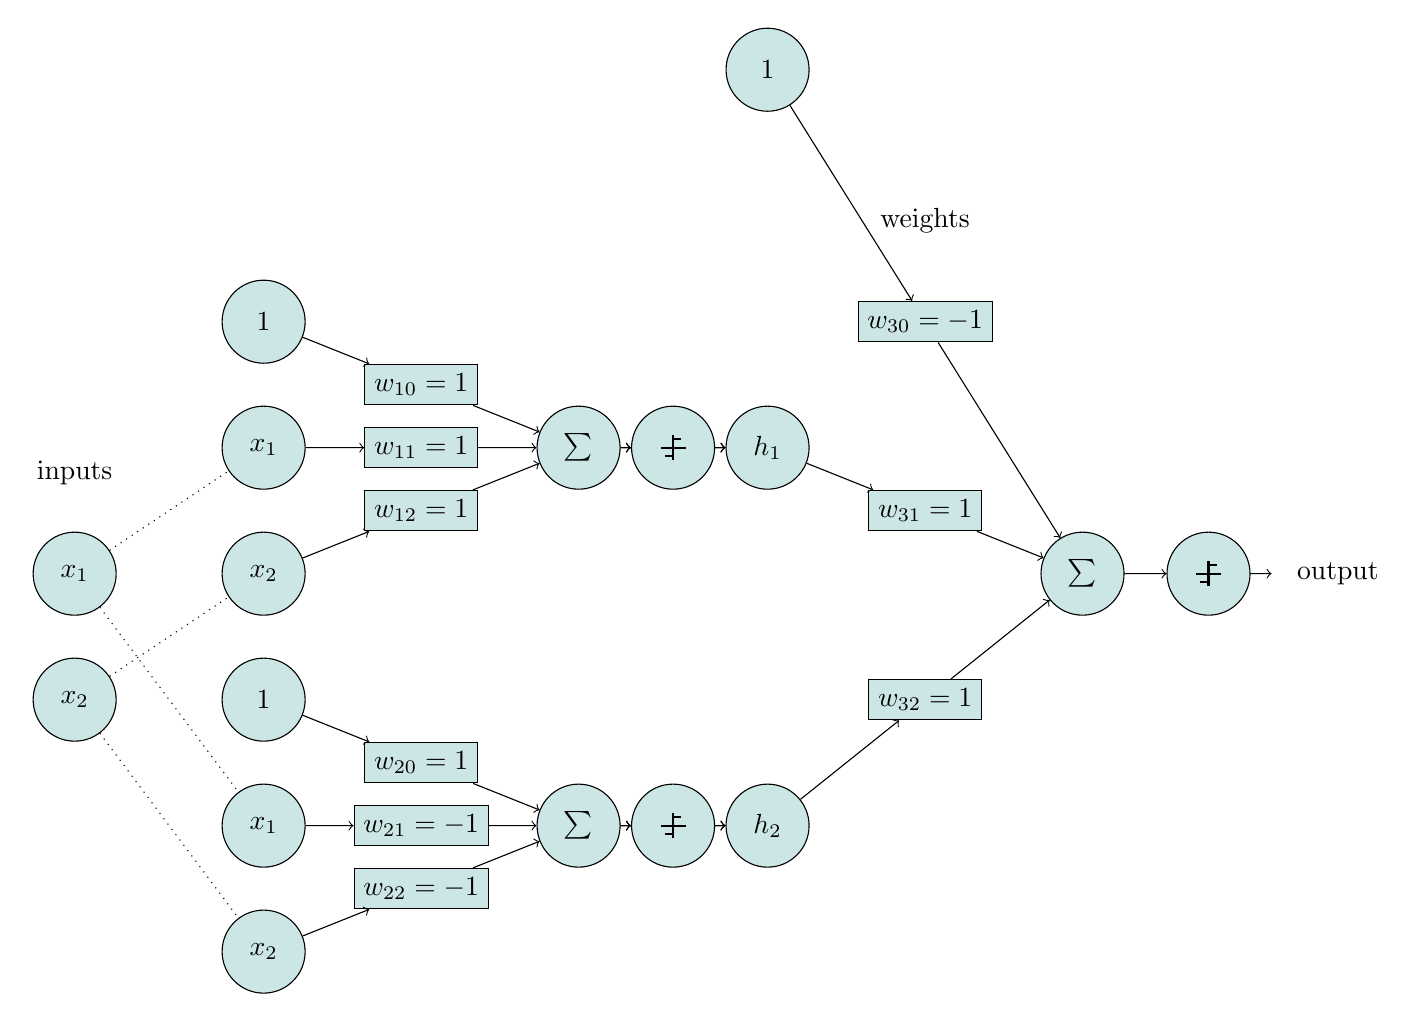
\begin{tikzpicture}[scale=0.8]

    %input x
    \node[input] (x1) at (-3,6){$x_1$};    
    \node[input] (x2) at (-3,4){$x_2$}; 

	% inputs of h1
    \foreach \h [count=\hi ] in {$x_2$,$x_1$,$1$}{
    	\node[input] (f1\hi) at (0,\hi*2cm +4cm) {\h};
    }
    % inputs of h2
    \foreach \h [count=\hi ] in {$x_2$,$x_1$,$1$}{
    	\node[input] (f2\hi) at (0,\hi*2cm -2cm) {\h};
    }
    
    \draw[dotted] (x1) -- (f12);    
    \draw[dotted] (x1) -- (f22);  
    \draw[dotted] (x2) -- (f11);    
    \draw[dotted] (x2) -- (f21);  
    
	% sum h1
	\node[functions] (sumh1) at (5,8) {$\sum$};
    % sum h2
	\node[functions] (sumh2) at (5,2) {$\sum$};
	
    \node[functions] (steph1) at (6.5,8) {};
       \begin{scope}[xshift=6.5cm,yshift=8cm,scale=.75]
         \addsymbol
       \end{scope}	
       
    \node[functions] (steph2) at (6.5,2) {};
       \begin{scope}[xshift=6.5cm,yshift=2cm,scale=.75]
         \addsymbol
       \end{scope}	
	
    % weights of h1
	\foreach \h [count=\hi ] in {$w_{12} =1$,$w_{11} = 1$,$w_{10} = 1$}{%
      	\path (f1\hi) -- node[weights] (w\hi) {\h} (sumh1);
      	\draw[->] (f1\hi) -- (w\hi);
      	\draw[->] (w\hi) -- (sumh1);
    } 
    % weights of h2
	\foreach \h [count=\hi ] in {$w_{22} =-1$,$w_{21} = -1$,$w_{20} = 1$}{%
      	\path (f2\hi) -- node[weights] (w\hi) {\h} (sumh2);
      	\draw[->] (f2\hi) -- (w\hi);
      	\draw[->] (w\hi) -- (sumh2);
    } 
	
	% inputs of g
	\foreach \h [count=\hi ] in {$h_2$,$h_1$,$1$}{%
      \node[input] (h\hi) at (8,\hi*6cm-4 cm) {\h};
    }
    % sum g
	\node[functions] (sumg) at (13,6) {$\sum$};
	% weights of g
	\foreach \h [count=\hi ] in {$w_{32} =1$,$w_{31} = 1$,$w_{30} = -1$}{%
      	\path (h\hi) -- node[weights] (w\hi) {\h} (sumg);
      	\draw[->] (h\hi) -- (w\hi);
      	\draw[->] (w\hi) -- (sumg);
      	\draw[->] (sumh1) -- (steph1);
      	\draw[->] (steph1) -- (h2);
      	\draw[->] (sumh2) -- (steph2);
      	\draw[->] (steph2) -- (h1);
    }        

    \node[functions] (stepg) at (15,6) {};
       \begin{scope}[xshift=15cm,yshift=6cm,scale=.75]
         \addsymbol
       \end{scope}
    
    \draw[->] (sumg) -- (stepg);       
	\draw[->] (stepg) -- ++(1,0);
	
	% Labels
	\node[above=1cm] at (x1) {inputs};
	\node[above=1cm] at (w3) {weights};
	\node[right=1cm] at (stepg) {output};
\end{tikzpicture}
\caption{Network for question 2c}
\label{fig2cc}
\end{figure}




























\section{Question 3}

\cite{rumel} is the original article introducing the Backpropagation algorithm. The URL for this document is in the reference.

\subsection{Question 3(a)}

We start with the following weights (Table \ref{table1}).

\begin{table}
\begin{tabular}{|c|c|c|c|c|c|c|c|c|c|}
\hline
$\omega_1$ & $\omega_2$ & $\omega_3$ & $\omega_4$ & $\omega_5$ & $\omega_6$ & $\omega_7$ & $\omega_8$ & $b_1$ & $b_2$\\
\hline
0.15 &0.2 &0.25 & 0.3 & 0.4 & 0.45 & 0.5 & 0.55 & 0.35 & 0.6 \\
\hline
\end{tabular}
\caption{Start weights}\label{table1}
\end{table}

\begin{table}
\begin{tabular}{|c|c|c|c|c|}
\hline
pattern & $x_1$ & $x_2$ & $d_1$ & $d_2$ \\
\hline
$p_1$ & 0.1 & 0.1 & 0.1 & 0.9 \\
$p_2$ & 0.1 & 0.9 & 0.9 & 0.1 \\
$p_3$ & 0.9 & 0.1 & 0.9 & 0.1 \\
$p_4$ & 0.9 & 0.9 & 0.1 & 0.9 \\
\hline
\end{tabular}
\caption{Input Patterns}\label{inputPatters}
\end{table}




\subsubsection{Pattern 1}
Doing the forward pass. Starting with the values on the hidden units
\begin{equation}
\begin{split}
net_{h1} &= \omega_1 x_1 + \omega_2 x_2 + b_1 \\
         &= 0.15(0.1) + 0.2(0.1) + 0.35 \\
         &= 0.385\\
\end{split}
\end{equation}

\begin{equation}
\begin{split}
out_{h1} &= \frac{1}{1+e^{-net_{h1}}}\\ 
         &= \frac{1}{1+e^{-0.385}}\\ 
         &= 0.595\\
\end{split}
\end{equation}

\begin{equation}
\begin{split}
net_{h2} &= \omega_3 x_1 + \omega_4 x_2 + b_1 \\
         &= 0.25(0.1) + 0.3(0.1) + 0.35 \\
         &= 0.405\\
\end{split}
\end{equation}

\begin{equation}
\begin{split}
out_{h2} &= \frac{1}{1+e^{-net_{h2}}}\\ 
         &= \frac{1}{1+e^{-0.405}}\\ 
         &= 0.6\\
\end{split}
\end{equation}

Continuing with the outputs of the network

\begin{equation}
\begin{split}
net_{o1} &= \omega_5 out_{h1} + \omega_6 out_{h2} + b_2 \\
         &= 0.4(0.595) + 0.45(0.6) + 0.6 \\
         &= 1.108\\
\end{split}
\end{equation}

\begin{equation}
\begin{split}
out_{o1} &= \frac{1}{1+e^{-net_{o1}}}\\ 
         &= \frac{1}{1+e^{-1.108}}\\ 
         &= 0.752\\
\end{split}
\end{equation}

\begin{equation}
\begin{split}
net_{02} &= \omega_7 out_{h1} + \omega_8 out_{h2} + b_2 \\
         &= 0.5(0.595) + 0.55(0.6) + 0.6 \\
         &= 1.227\\
\end{split}
\end{equation}

\begin{equation}
\begin{split}
out_{o1} &= \frac{1}{1+e^{-net_{h1}}}\\ 
         &= \frac{1}{1+e^{-1.223}}\\ 
         &= 0.773\\
\end{split}
\end{equation}






















Now we need to calculate the error

\begin{equation}
\begin{split}
E_{total} &= E_{o1} + E_{02} \\
          &= \frac{1}{2}(0.1-0.752)^2 + \frac{1}{2}(0.9 - 0.773)^2 \\
          &= 0.220 \\
\end{split}
\end{equation}

\begin{equation}
\begin{split}
\delta_{o1} &= -(target_{o1} -out_{o1})(out_{o1})(1-out_{o1})\\
            &= -(0.1-0.752)(0.752)(1-0.752)\\
            &= 0.122\\
\end{split}
\end{equation}

\begin{equation}
\begin{split}
\pdv{E_{total}}{\omega_5} &= \delta_{o1}out_{h1}\\
                          &= 0.122(0.595)\\
                          &= 0.073\\
\end{split}
\end{equation}

We calculate the new value for $\omega_5$
\begin{equation}
\begin{split}
\omega_5^1 &= \omega_5^0 - \eta\pdv{E_{total}}{\omega_5}\\
           &= 0.4 -0.5(0.073)\\
           &= 0.364\\
\end{split}
\end{equation}

\begin{equation}
\begin{split}
\pdv{E_{total}}{\omega_6} &= \delta_{o1}out_{h2}\\
                          &= 0.122(0.6)\\
                          &= 0.073\\
\end{split}
\end{equation}

We calculate the new value for $\omega_6$
\begin{equation}
\begin{split}
\omega_6^1 &= \omega_6^0 - \eta\pdv{E_{total}}{\omega_6}\\
           &= 0.45 -0.5(0.073)\\
           &= 0.414\\
\end{split}
\end{equation}

\begin{equation}
\begin{split}
\delta_{o2} &= -(target_{o2} -out_{o2})(out_{o2})(1-out_{o2})\\
            &= -(0.9-0.773)(0.773)(1-0.773)\\
            &= -0.022\\
\end{split}
\end{equation}

\begin{equation}
\begin{split}
\pdv{E_{total}}{\omega_7} &= \delta_{o2}out_{h1}\\
                          &= -0.022(0.595)\\
                          &= -0.013\\
\end{split}
\end{equation}

We calculate the new value for $\omega_7$
\begin{equation}
\begin{split}
\omega_7^1 &= \omega_7^0 - \eta\pdv{E_{total}}{\omega_7}\\
           &= 0.5 -0.5(-0.013)\\
           &= 0.507\\
\end{split}
\end{equation}

\begin{equation}
\begin{split}
\pdv{E_{total}}{\omega_8} &= \delta_{o2}out_{h2}\\
                          &= -0.022(0.6)\\
                          &= -0.013\\
\end{split}
\end{equation}

We calculate the new value for $\omega_8$
\begin{equation}
\begin{split}
\omega_8^1 &= \omega_8^0 - \eta\pdv{E_{total}}{\omega_8}\\
           &= 0.55 -0.5(-0.013)\\
           &= 0.557\\
\end{split}
\end{equation}







Now we need to pass the error back to the hidden units

\begin{equation}
\begin{split}
\delta_{h1} &= (\delta_{o1}\omega_5^0 + \delta_{o2}\omega_7^0)(out_{h1})(1-out_{h1})\\
&= (0.122(0.4) -0.022(0.5))(0.595)(1-0.595)\\
&= 0.009\\
\end{split}
\end{equation}

\begin{equation}
\begin{split}
\pdv{E_{total}}{\omega_1} &= \delta_{h1}x_1\\ 
                          &= 0.009(0.1)\\
                          &= 0.001\\
\end{split}
\end{equation}

\begin{equation}
\begin{split}
\omega_1^1 &= \omega_1^0 - \eta\pdv{E_{total}}{\omega_1}\\
           &= 0.15 -0.5(0.001)\\
           &= 0.149\\
\end{split}
\end{equation}

\begin{equation}
\begin{split}
\pdv{E_{total}}{\omega_2} &= \delta_{h1}x_2\\ 
                          &= 0.009(0.1)\\
                          &= 0.001\\
\end{split}
\end{equation}

\begin{equation}
\begin{split}
\omega_2^1 &= \omega_2^0 - \eta\pdv{E_{total}}{\omega_2}\\
           &= 0.2 -0.5(0.001)\\
           &= 0.199\\
\end{split}
\end{equation}

\begin{equation}
\begin{split}
\delta_{h2} &= (\delta_{o1}\omega_6^0 + \delta_{o2}\omega_8^0)(out_{h2})(1-out_{h2})\\
&= (0.122(0.45) -0.022(0.55))(0.6)(1-0.6)\\
&= 0.010\\
\end{split}
\end{equation}

\begin{equation}
\begin{split}
\pdv{E_{total}}{\omega_3} &= \delta_{h2}x_1\\ 
                          &= 0.010(0.1)\\
                          &= 0.001\\
\end{split}
\end{equation}

\begin{equation}
\begin{split}
\omega_3^1 &= \omega_3^0 - \eta\pdv{E_{total}}{\omega_3}\\
           &= 0.25 -0.5(0.001)\\
           &= 0.249\\
\end{split}
\end{equation}

\begin{equation}
\begin{split}
\pdv{E_{total}}{\omega_4} &= \delta_{h2}x_2\\ 
                          &= 0.010(0.1)\\
                          &= 0.001\\
\end{split}
\end{equation}

\begin{equation}
\begin{split}
\omega_4^1 &= \omega_4^0 - \eta\pdv{E_{total}}{\omega_4}\\
           &= 0.3 -0.5(0.001)\\
           &= 0.299\\
\end{split}
\end{equation}

\subsubsection{Pattern 2}
\begin{table}
\begin{tabular}{|c|c|c|c|c|c|c|c|c|c|}
\hline
$\omega_1$ & $\omega_2$ & $\omega_3$ & $\omega_4$ & $\omega_5$ & $\omega_6$ & $\omega_7$ & $\omega_8$ & $b_1$ & $b_2$\\
\hline
0.149 &0.199 &0.249 & 0.299 & 0.364 & 0.414 & 0.507 & 0.557 & 0.35 & 0.6 \\
\hline
\end{tabular}
\caption{Weights after applying pattern 1}\label{tablep2}
\end{table}

Continuing with the forward pass for pattern 2

\begin{equation}
\begin{split}
net_{h1} &= \omega_1 x_1 + \omega_2 x_2 + b_1 \\
         &= 0.149(0.1) + 0.199(0.9) + 0.35 \\
         &= 0.544\\
\end{split}
\end{equation}

\begin{equation}
\begin{split}
out_{h1} &= \frac{1}{1+e^{-net_{h1}}}\\ 
         &= \frac{1}{1+e^{-0.544}}\\ 
         &= 0.633\\
\end{split}
\end{equation}

\begin{equation}
\begin{split}
net_{h2} &= \omega_3 x_1 + \omega_4 x_2 + b_1 \\
         &= 0.249(0.1) + 0.299(0.9) + 0.35 \\
         &= 0.644\\
\end{split}
\end{equation}

\begin{equation}
\begin{split}
out_{h2} &= \frac{1}{1+e^{-net_{h2}}}\\ 
         &= \frac{1}{1+e^{-0.644}}\\ 
         &= 0.656\\
\end{split}
\end{equation}

Continuing with the outputs of the network

\begin{equation}
\begin{split}
net_{o1} &= \omega_5 out_{h1} + \omega_6 out_{h2} + b_2 \\
         &= 0.364(0.633) + 0.414(0.656) + 0.6 \\
         &= 1.102\\
\end{split}
\end{equation}

\begin{equation}
\begin{split}
out_{o1} &= \frac{1}{1+e^{-net_{o1}}}\\ 
         &= \frac{1}{1+e^{-1.102}}\\ 
         &= 0.751\\
\end{split}
\end{equation}

\begin{equation}
\begin{split}
net_{02} &= \omega_7 out_{h1} + \omega_8 out_{h2} + b_2 \\
         &= 0.507(0.633) + 0.557(0.644) + 0.6 \\
         &= 1.280\\
\end{split}
\end{equation}

\begin{equation}
\begin{split}
out_{o1} &= \frac{1}{1+e^{-net_{h1}}}\\ 
         &= \frac{1}{1+e^{-1.280}}\\ 
         &= 0.782\\
\end{split}
\end{equation}

Now we need to calculate the error

\begin{equation}
\begin{split}
E_{total} &= E_{o1} + E_{02} \\
          &= \frac{1}{2}(0.9-0.751)^2 + \frac{1}{2}(0.1 - 0.782)^2 \\
          &= 0.244 \\
\end{split}
\end{equation}

\begin{equation}
\begin{split}
\delta_{o1} &= -(target_{o1} -out_{o1})(out_{o1})(1-out_{o1})\\
            &= -(0.9-0.751)(0.751)(1-0.751)\\
            &= -0.028\\
\end{split}
\end{equation}

\begin{equation}
\begin{split}
\pdv{E_{total}}{\omega_5} &= \delta_{o1}out_{h1}\\
                          &= -0.028(0.633)\\
                          &= -0.018\\
\end{split}
\end{equation}

We calculate the new value for $\omega_5$
\begin{equation}
\begin{split}
\omega_5^2 &= \omega_5^1 - \eta\pdv{E_{total}}{\omega_5}\\
           &= 0.364 -0.5(-0.018)\\
           &= 0.373\\
\end{split}
\end{equation}

\begin{equation}
\begin{split}
\pdv{E_{total}}{\omega_6} &= \delta_{o1}out_{h2}\\
                          &= -0.028(0.656)\\
                          &= -0.018\\
\end{split}
\end{equation}

We calculate the new value for $\omega_6$
\begin{equation}
\begin{split}
\omega_6^2 &= \omega_6^1 - \eta\pdv{E_{total}}{\omega_6}\\
           &= 0.414 -0.5(-0.018)\\
           &= 0.423\\
\end{split}
\end{equation}

\begin{equation}
\begin{split}
\delta_{o2} &= -(target_{o2} -out_{o2})(out_{o2})(1-out_{o2})\\
            &= -(0.1-0.782)(0.782)(1-0.782)\\
            &= 0.166\\
\end{split}
\end{equation}

\begin{equation}
\begin{split}
\pdv{E_{total}}{\omega_7} &= \delta_{o2}out_{h1}\\
                          &= 0.166(0.633)\\
                          &= 0.073\\
\end{split}
\end{equation}

We calculate the new value for $\omega_7$
\begin{equation}
\begin{split}
\omega_7^2 &= \omega_7^1 - \eta\pdv{E_{total}}{\omega_7}\\
           &= 0.507 -0.5(0.073)\\
           &= 0.471\\
\end{split}
\end{equation}

\begin{equation}
\begin{split}
\pdv{E_{total}}{\omega_8} &= \delta_{o2}out_{h2}\\
                          &= 0.166(0.656)\\
                          &= 0.076\\
\end{split}
\end{equation}

We calculate the new value for $\omega_8$
\begin{equation}
\begin{split}
\omega_8^2 &= \omega_8^1 - \eta\pdv{E_{total}}{\omega_8}\\
           &= 0.557 -0.5(0.076)\\
           &= 0.519\\
\end{split}
\end{equation}







Now we need to pass the error back to the hidden units

\begin{equation}
\begin{split}
\delta_{h1} &= (\delta_{o1}\omega_5^1 + \delta_{o2}\omega_7^1)(out_{h1})(1-out_{h1})\\
&= (-0.028(0.364) +0.116(0.507))(0.507)(1-0.507)\\
&= 0.011\\
\end{split}
\end{equation}

\begin{equation}
\begin{split}
\pdv{E_{total}}{\omega_1} &= \delta_{h1}x_1\\ 
                          &= 0.011(0.1)\\
                          &= 0.001\\
\end{split}
\end{equation}

\begin{equation}
\begin{split}
\omega_1^2 &= \omega_1^1 - \eta\pdv{E_{total}}{\omega_1}\\
           &= 0.149 -0.5(0.001)\\
           &= 0.149\\
\end{split}
\end{equation}

\begin{equation}
\begin{split}
\pdv{E_{total}}{\omega_2} &= \delta_{h1}x_2\\ 
                          &= 0.011(0.9)\\
                          &= 0.010\\
\end{split}
\end{equation}

\begin{equation}
\begin{split}
\omega_2^2 &= \omega_2^1 - \eta\pdv{E_{total}}{\omega_2}\\
           &= 0.199 -0.5(0.010)\\
           &= 0.194\\
\end{split}
\end{equation}

\begin{equation}
\begin{split}
\delta_{h2} &= (\delta_{o1}\omega_6^1 + \delta_{o2}\omega_8^1)(out_{h2})(1-out_{h2})\\
&= (-0.028(0.414) + 0.116(0.557))(0.656)(1-0.656)\\
&= 0.012\\
\end{split}
\end{equation}

\begin{equation}
\begin{split}
\pdv{E_{total}}{\omega_3} &= \delta_{h2}x_1\\ 
                          &= 0.012(0.1)\\
                          &= 0.001\\
\end{split}
\end{equation}

\begin{equation}
\begin{split}
\omega_3^2 &= \omega_3^1 - \eta\pdv{E_{total}}{\omega_3}\\
           &= 0.249 -0.5(0.001)\\
           &= 0.249\\
\end{split}
\end{equation}

\begin{equation}
\begin{split}
\pdv{E_{total}}{\omega_4} &= \delta_{h2}x_2\\ 
                          &= 0.012(0.9)\\
                          &= 0.011\\
\end{split}
\end{equation}

\begin{equation}
\begin{split}
\omega_4^2 &= \omega_4^1 - \eta\pdv{E_{total}}{\omega_4}\\
           &= 0.299 -0.5(0.011)\\
           &= 0.294\\
\end{split}
\end{equation}

\subsubsection{Pattern 3}
\begin{table}
\begin{tabular}{|c|c|c|c|c|c|c|c|c|c|}
\hline
$\omega_1$ & $\omega_2$ & $\omega_3$ & $\omega_4$ & $\omega_5$ & $\omega_6$ & $\omega_7$ & $\omega_8$ & $b_1$ & $b_2$\\
\hline
0.149 &0.194 &0.249 & 0.294 & 0.373 & 0.423 & 0.471 & 0.519 & 0.35 & 0.6 \\
\hline
\end{tabular}
\caption{Weights after applying pattern 2}\label{tablep3}
\end{table}

Continuing with the forward pass for pattern 3

\begin{equation}
\begin{split}
net_{h1} &= \omega_1 x_1 + \omega_2 x_2 + b_1 \\
         &= 0.149(0.9) + 0.194(0.1) + 0.35 \\
         &= 0.504\\
\end{split}
\end{equation}

\begin{equation}
\begin{split}
out_{h1} &= \frac{1}{1+e^{-net_{h1}}}\\ 
         &= \frac{1}{1+e^{-0.504}}\\ 
         &= 0.623\\
\end{split}
\end{equation}

\begin{equation}
\begin{split}
net_{h2} &= \omega_3 x_1 + \omega_4 x_2 + b_1 \\
         &= 0.249(0.9) + 0.294(0.1) + 0.35 \\
         &= 0.604\\
\end{split}
\end{equation}

\begin{equation}
\begin{split}
out_{h2} &= \frac{1}{1+e^{-net_{h2}}}\\ 
         &= \frac{1}{1+e^{-0.604}}\\ 
         &= 0.646\\
\end{split}
\end{equation}

Continuing with the outputs of the network

\begin{equation}
\begin{split}
net_{o1} &= \omega_5 out_{h1} + \omega_6 out_{h2} + b_2 \\
         &= 0.373(0.623) + 0.423(0.646) + 0.6 \\
         &= 1.106\\
\end{split}
\end{equation}

\begin{equation}
\begin{split}
out_{o1} &= \frac{1}{1+e^{-net_{o1}}}\\ 
         &= \frac{1}{1+e^{-1.106}}\\ 
         &= 0.751\\
\end{split}
\end{equation}

\begin{equation}
\begin{split}
net_{02} &= \omega_7 out_{h1} + \omega_8 out_{h2} + b_2 \\
         &= 0.471(0.623) + 0.519(0.646) + 0.6 \\
         &= 1.229\\
\end{split}
\end{equation}

\begin{equation}
\begin{split}
out_{o1} &= \frac{1}{1+e^{-net_{h1}}}\\ 
         &= \frac{1}{1+e^{-1.229}}\\ 
         &= 0.774\\
\end{split}
\end{equation}

Now we need to calculate the error

\begin{equation}
\begin{split}
E_{total} &= E_{o1} + E_{02} \\
          &= \frac{1}{2}(0.9-0.751)^2 + \frac{1}{2}(0.1 - 0.774)^2 \\
          &= 0.238 \\
\end{split}
\end{equation}

\begin{equation}
\begin{split}
\delta_{o1} &= -(target_{o1} -out_{o1})(out_{o1})(1-out_{o1})\\
            &= -(0.9-0.751)(0.751)(1-0.751)\\
            &= -0.028\\
\end{split}
\end{equation}

\begin{equation}
\begin{split}
\pdv{E_{total}}{\omega_5} &= \delta_{o1}out_{h1}\\
                          &= -0.028(0.623)\\
                          &= -0.017\\
\end{split}
\end{equation}

We calculate the new value for $\omega_5$
\begin{equation}
\begin{split}
\omega_5^3 &= \omega_5^2 - \eta\pdv{E_{total}}{\omega_5}\\
           &= 0.373 -0.5(-0.017)\\
           &= 0.382\\
\end{split}
\end{equation}

\begin{equation}
\begin{split}
\pdv{E_{total}}{\omega_6} &= \delta_{o1}out_{h2}\\
                          &= -0.028(0.646)\\
                          &= -0.018\\
\end{split}
\end{equation}

We calculate the new value for $\omega_6$
\begin{equation}
\begin{split}
\omega_6^3 &= \omega_6^2 - \eta\pdv{E_{total}}{\omega_6}\\
           &= 0.423 -0.5(-0.018)\\
           &= 0.432\\
\end{split}
\end{equation}

\begin{equation}
\begin{split}
\delta_{o2} &= -(target_{o2} -out_{o2})(out_{o2})(1-out_{o2})\\
            &= -(0.1-0.774)(0.774)(1-0.774)\\
            &= 0.118\\
\end{split}
\end{equation}

\begin{equation}
\begin{split}
\pdv{E_{total}}{\omega_7} &= \delta_{o2}out_{h1}\\
                          &= 0.118(0.623)\\
                          &= 0.074\\
\end{split}
\end{equation}

We calculate the new value for $\omega_7$
\begin{equation}
\begin{split}
\omega_7^3 &= \omega_7^2 - \eta\pdv{E_{total}}{\omega_7}\\
           &= 0.471 -0.5(0.074)\\
           &= 0.434\\
\end{split}
\end{equation}

\begin{equation}
\begin{split}
\pdv{E_{total}}{\omega_8} &= \delta_{o2}out_{h2}\\
                          &= 0.118(0.646)\\
                          &= 0.077\\
\end{split}
\end{equation}

We calculate the new value for $\omega_8$
\begin{equation}
\begin{split}
\omega_8^3 &= \omega_8^2 - \eta\pdv{E_{total}}{\omega_8}\\
           &= 0.519 -0.5(0.077)\\
           &= 0.480\\
\end{split}
\end{equation}







Now we need to pass the error back to the hidden units

\begin{equation}
\begin{split}
\delta_{h1} &= (\delta_{o1}\omega_5^2 + \delta_{o2}\omega_7^2)(out_{h1})(1-out_{h1})\\
&= (-0.028(0.373) +0.118(0.471))(0.623)(1-0.623)\\
&= 0.011\\
\end{split}
\end{equation}

\begin{equation}
\begin{split}
\pdv{E_{total}}{\omega_1} &= \delta_{h1}x_1\\ 
                          &= 0.011(0.9)\\
                          &= 0.010\\
\end{split}
\end{equation}

\begin{equation}
\begin{split}
\omega_1^3 &= \omega_1^2 - \eta\pdv{E_{total}}{\omega_1}\\
           &= 0.149 -0.5(0.010)\\
           &= 0.144\\
\end{split}
\end{equation}

\begin{equation}
\begin{split}
\pdv{E_{total}}{\omega_2} &= \delta_{h1}x_2\\ 
                          &= 0.011(0.1)\\
                          &= 0.001\\
\end{split}
\end{equation}

\begin{equation}
\begin{split}
\omega_2^3 &= \omega_2^2 - \eta\pdv{E_{total}}{\omega_2}\\
           &= 0.194 -0.5(0.001)\\
           &= 0.194\\
\end{split}
\end{equation}

\begin{equation}
\begin{split}
\delta_{h2} &= (\delta_{o1}\omega_6^2 + \delta_{o2}\omega_8^2)(out_{h2})(1-out_{h2})\\
&= (-0.028(0.423) + 0.118(0.519))(0.646)(1-0.646)\\
&= 0.011\\
\end{split}
\end{equation}

\begin{equation}
\begin{split}
\pdv{E_{total}}{\omega_3} &= \delta_{h2}x_1\\ 
                          &= 0.011(0.9)\\
                          &= 0.010\\
\end{split}
\end{equation}

\begin{equation}
\begin{split}
\omega_3^3 &= \omega_3^2 - \eta\pdv{E_{total}}{\omega_3}\\
           &= 0.249 -0.5(0.010)\\
           &= 0.244\\
\end{split}
\end{equation}

\begin{equation}
\begin{split}
\pdv{E_{total}}{\omega_4} &= \delta_{h2}x_2\\ 
                          &= 0.011(0.1)\\
                          &= 0.001\\
\end{split}
\end{equation}

\begin{equation}
\begin{split}
\omega_4^3 &= \omega_4^2 - \eta\pdv{E_{total}}{\omega_4}\\
           &= 0.294 -0.5(0.001)\\
           &= 0.294\\
\end{split}
\end{equation}

\subsubsection{Pattern 4}
\begin{table}
\begin{tabular}{|c|c|c|c|c|c|c|c|c|c|}
\hline
$\omega_1$ & $\omega_2$ & $\omega_3$ & $\omega_4$ & $\omega_5$ & $\omega_6$ & $\omega_7$ & $\omega_8$ & $b_1$ & $b_2$\\
\hline
0.144 &0.194 &0.244 & 0.294 & 0.382 & 0.432 & 0.434 & 0.480 & 0.35 & 0.6 \\
\hline
\end{tabular}
\caption{Weights after applying pattern 3}\label{tablep4}
\end{table}

Continuing with the forward pass for pattern 4

\begin{equation}
\begin{split}
net_{h1} &= \omega_1 x_1 + \omega_2 x_2 + b_1 \\
         &= 0.144(0.9) + 0.194(0.9) + 0.35 \\
         &= 0.654\\
\end{split}
\end{equation}

\begin{equation}
\begin{split}
out_{h1} &= \frac{1}{1+e^{-net_{h1}}}\\ 
         &= \frac{1}{1+e^{-0.654}}\\ 
         &= 0.658\\
\end{split}
\end{equation}

\begin{equation}
\begin{split}
net_{h2} &= \omega_3 x_1 + \omega_4 x_2 + b_1 \\
         &= 0.244(0.9) + 0.294(0.9) + 0.35 \\
         &= 0.834\\
\end{split}
\end{equation}

\begin{equation}
\begin{split}
out_{h2} &= \frac{1}{1+e^{-net_{h2}}}\\ 
         &= \frac{1}{1+e^{-0.834}}\\ 
         &= 0.697\\
\end{split}
\end{equation}

Continuing with the outputs of the network

\begin{equation}
\begin{split}
net_{o1} &= \omega_5 out_{h1} + \omega_6 out_{h2} + b_2 \\
         &= 0.382(0.658) + 0.432(0.697) + 0.6 \\
         &= 1.152\\
\end{split}
\end{equation}

\begin{equation}
\begin{split}
out_{o1} &= \frac{1}{1+e^{-net_{o1}}}\\ 
         &= \frac{1}{1+e^{-1.152}}\\ 
         &= 0.760\\
\end{split}
\end{equation}

\begin{equation}
\begin{split}
net_{02} &= \omega_7 out_{h1} + \omega_8 out_{h2} + b_2 \\
         &= 0.434(0.658) + 0.480(0.697) + 0.6 \\
         &= 1.220\\
\end{split}
\end{equation}

\begin{equation}
\begin{split}
out_{o1} &= \frac{1}{1+e^{-net_{h1}}}\\ 
         &= \frac{1}{1+e^{-1.220}}\\ 
         &= 0.772\\
\end{split}
\end{equation}

Now we need to calculate the error

\begin{equation}
\begin{split}
E_{total} &= E_{o1} + E_{02} \\
          &= \frac{1}{2}(0.1-0.760)^2 + \frac{1}{2}(0.9 - 0.772)^2 \\
          &= 0.226 \\
\end{split}
\end{equation}

\begin{equation}
\begin{split}
\delta_{o1} &= -(target_{o1} -out_{o1})(out_{o1})(1-out_{o1})\\
            &= -(0.1-0.760)(0.760)(1-0.760)\\
            &= 0.120\\
\end{split}
\end{equation}

\begin{equation}
\begin{split}
\pdv{E_{total}}{\omega_5} &= \delta_{o1}out_{h1}\\
                          &= 0.120(0.658)\\
                          &= 0.079\\
\end{split}
\end{equation}

We calculate the new value for $\omega_5$
\begin{equation}
\begin{split}
\omega_5^4 &= \omega_5^3 - \eta\pdv{E_{total}}{\omega_5}\\
           &= 0.382 -0.5(0.079)\\
           &= 0.342\\
\end{split}
\end{equation}

\begin{equation}
\begin{split}
\pdv{E_{total}}{\omega_6} &= \delta_{o1}out_{h2}\\
                          &= 0.120(0.697)\\
                          &= 0.084\\
\end{split}
\end{equation}

We calculate the new value for $\omega_6$
\begin{equation}
\begin{split}
\omega_6^4 &= \omega_6^3 - \eta\pdv{E_{total}}{\omega_6}\\
           &= 0.432 -0.5(0.084)\\
           &= 0.390\\
\end{split}
\end{equation}

\begin{equation}
\begin{split}
\delta_{o2} &= -(target_{o2} -out_{o2})(out_{o2})(1-out_{o2})\\
            &= -(0.9-0.772)(0.772)(1-0.772)\\
            &= -0.023\\
\end{split}
\end{equation}

\begin{equation}
\begin{split}
\pdv{E_{total}}{\omega_7} &= \delta_{o2}out_{h1}\\
                          &= -0.023(0.658)\\
                          &= -0.015\\
\end{split}
\end{equation}

We calculate the new value for $\omega_7$
\begin{equation}
\begin{split}
\omega_7^4 &= \omega_7^3 - \eta\pdv{E_{total}}{\omega_7}\\
           &= 0.434 -0.5(-0.015)\\
           &= 0.441\\
\end{split}
\end{equation}

\begin{equation}
\begin{split}
\pdv{E_{total}}{\omega_8} &= \delta_{o2}out_{h2}\\
                          &= -0.023(0.697)\\
                          &= -0.016\\
\end{split}
\end{equation}

We calculate the new value for $\omega_8$
\begin{equation}
\begin{split}
\omega_8^4 &= \omega_8^3 - \eta\pdv{E_{total}}{\omega_8}\\
           &= 0.480 -0.5(-0.016)\\
           &= 0.488\\
\end{split}
\end{equation}







Now we need to pass the error back to the hidden units

\begin{equation}
\begin{split}
\delta_{h1} &= (\delta_{o1}\omega_5^3 + \delta_{o2}\omega_7^3)(out_{h1})(1-out_{h1})\\
&= (0.120(0.382) -0.023(0.434))(0.658)(1-0.658)\\
&= 0.008\\
\end{split}
\end{equation}

\begin{equation}
\begin{split}
\pdv{E_{total}}{\omega_1} &= \delta_{h1}x_1\\ 
                          &= 0.008(0.9)\\
                          &= 0.007\\
\end{split}
\end{equation}

\begin{equation}
\begin{split}
\omega_1^4 &= \omega_1^3 - \eta\pdv{E_{total}}{\omega_1}\\
           &= 0.144 -0.5(0.007)\\
           &= 0.141\\
\end{split}
\end{equation}

\begin{equation}
\begin{split}
\pdv{E_{total}}{\omega_2} &= \delta_{h1}x_2\\ 
                          &= 0.008(0.9)\\
                          &= 0.007\\
\end{split}
\end{equation}

\begin{equation}
\begin{split}
\omega_2^4 &= \omega_2^3 - \eta\pdv{E_{total}}{\omega_2}\\
           &= 0.194 -0.5(0.007)\\
           &= 0.191\\
\end{split}
\end{equation}

\begin{equation}
\begin{split}
\delta_{h2} &= (\delta_{o1}\omega_6^3 + \delta_{o2}\omega_8^3)(out_{h2})(1-out_{h2})\\
&= (0.120(0.432) -0.023(0.480))(0.697)(1-0.697)\\
&= 0.009\\
\end{split}
\end{equation}

\begin{equation}
\begin{split}
\pdv{E_{total}}{\omega_3} &= \delta_{h2}x_1\\ 
                          &= 0.009(0.9)\\
                          &= 0.008\\
\end{split}
\end{equation}

\begin{equation}
\begin{split}
\omega_3^4 &= \omega_3^3 - \eta\pdv{E_{total}}{\omega_3}\\
           &= 0.244 -0.5(0.008)\\
           &= 0.240\\
\end{split}
\end{equation}

\begin{equation}
\begin{split}
\pdv{E_{total}}{\omega_4} &= \delta_{h2}x_2\\ 
                          &= 0.009(0.9)\\
                          &= 0.008\\
\end{split}
\end{equation}

\begin{equation}
\begin{split}
\omega_4^3 &= \omega_4^2 - \eta\pdv{E_{total}}{\omega_4}\\
           &= 0.294 -0.5(0.008)\\
           &= 0.290\\
\end{split}
\end{equation}

\begin{table}
\begin{tabular}{|c|c|c|c|c|c|c|c|c|c|}
\hline
$\omega_1$ & $\omega_2$ & $\omega_3$ & $\omega_4$ & $\omega_5$ & $\omega_6$ & $\omega_7$ & $\omega_8$ & $b_1$ & $b_2$\\
\hline
0.141 &0.191 &0.240 & 0.290 & 0.342 & 0.390 & 0.441 & 0.488 & 0.35 & 0.6 \\
\hline
\end{tabular}
\caption{Weights after applying pattern 4}\label{tablep5}
\end{table}


The resultant weights after all 4 patters can be found in Table \ref{tablep5}









\subsection{Question 3(b)}

According to \cite{Michell2009} the following functions can be modeled by feed forward networks. Firstly any boolean function can be represented by using 2 layers of units (not counting the input layer). But, in the worst case, the number of hidden unit will grow exponentially with the number of inputs. Secondly any Continuous bounded function can be modeled to an arbitrary level of accuracy with a network with one hidden layer. Thirdly any arbitrary function can be approximated with a network containing 2 layers of hidden units.
 
\subsection{Question 3(c)}

The error surface for multi-layered networks contains multiple local minima. The gradient descent method used can only converge to a local minima which is not necessarily the global minimum. When the gradient decent process starts close to a local minimum the algorithm will follow the gradient to the local minimum  \citep{Michell2009}.

Networks with higher dimensions may suffer less from local minima because when the network reaches a local minimum in a certain dimension, the other dimensions are not necessarily at a minimum. Their weights can get the network out of some local minima  \citep{Michell2009}.
 
The problem of local minima can also lessened by using a momentum term. As in

\begin{equation}
\begin{split}
\omega_i^{j+1} &= \omega_i^j - \eta\pdv{E_{total}}{\omega_i^j} +\alpha (\omega_i^{j}-\omega_i^{j-1})
\end{split}
\end{equation}

where alpha is the momentum constant and this depends on the previous change in the weight. This way the algorithm can get out of a relatively small local minimum \citep{Michell2009}.

One technique is so called "on-line training". Here the weights are updated after each pattern is processed rather than batch or off-line where the weights are updated after all the patterns are processed. On-line training can add noise to the gradient direction and thereby avoiding some shallow local minima \citep{rojas}.

Another method is simulated annealing \citep{rojas};


\subsection{Question 3(d)}

A discussion of the identity function can be found in \citep[p106]{Michell2009} at $http://www.cs.ubbcluj.ro/\sim gabis/ml/ml-books/McGrawHill - Machine Learning -Tom Mitchell.pdf$

Using a 8 X 3 X 8 network we want to represent the identity function. In other words when any input node is given an high input we want the corresponding output node to be high. Thus if input 2 is high and all the other nodes are low (01000000), output 2 needs to be high and all other outputs low (01000000).  The problem is that there is not enough nodes in the hidden layer to simply forward the value from the input node to the corresponding output node. 

When we attempt to train such a network the network finds a representation in the hidden layer to represent all 8 inputs. The network uses a binary representation where the input (00100000) will be represented as (011) in the hidden units. This will then be output as (00100000). This way the network learn a new representation that it was not explicitly told.

The values from the book can be found in table \ref{table2}

\begin{table}
\begin{tabular}{|c|c|c|c|c||}
\hline
$Input$ & $h_1$ & $h_2$ & $h_3$ & $Output$ \\
\hline
10000000 & 0.89 & 0.04 & 0.08 & 10000000 \\
01000000 & 0.15 & 0.99 & 0.99 & 01000000 \\
00100000 & 0.01 & 0.97 & 0.27 & 00100000 \\
00010000 & 0.99 & 0.97 & 0.71 & 00010000 \\
00001000 & 0.03 & 0.05 & 0.02 & 00001000 \\
00000100 & 0.01 & 0.11 & 0.88 & 00000100 \\
00000010 & 0.80 & 0.01 & 0.98 & 00000010 \\
00000001 & 0.60 & 0.94 & 0.01 & 00000001 \\
\hline
\end{tabular}
\caption{Hidden unit representation}\label{table2}
\end{table}

\subsection{Question 3(e)}

The sigmoid function is defined as

\begin{equation}
\sigma(y) = \frac{1}{1+e^{-y}}
\end{equation}

Firstly the output of this activation function is continuous. This makes it easier to connect multiple neurons together and weight different inputs form different neurons. The function is also easily differentiable. Secondly because the function is very steep it tends to force values to be high or low. Which makes it suitable as a classifier. Thirdly because the output of the sigmoid is always bound, our function wont grow out of bounds \citep{AvinashSharmaV2017}.

Another possibility is the $tanh$ function \citep{C.M.Bishop,AvinashSharmaV2017}.

\begin{equation}
\begin{split}
f(x) &= tanh(x)\\
     &= \frac{2}{1-e^{-2x}} - 1
\end{split}
\end{equation}

As we can see the $tanh$ function is very similar to the sigmoid function and has thus most of the same advantages. But the angle of $tanh$ is steeper than the sigmoid function. 

Another possibility is the linear function.

\begin{equation}
f(x) = mx+c 
\end{equation}

The problem with the linear function is that stacking multiple neurons is always equivalent to 1 linear function. Thus we lose the ability to classify with multiple neurons. Also the derivative of a linear function is not a function of x. Thus the backpropagation step will always make a constant step. This is not desirable.
\bibliography{mybib}
\end{document}
